\section{Model}
\label{sec:model}

\pldone{I'd start out with the overarching problem setting \emph{independent} of our approach.
  Since this is a novel setting, let's make it objective; you don't have to use Bayesian decision theory
  to solve it.
In particular, talk about the inputs, the outputs, the measurements, the online setting, latency, cost, etc.,
but no model, no algorithms.
}{see below}

Let us formalize our problem setting. %, using the disaster relief example from the introduction to make things concrete.
We receive a stream of inputs $\bx\oft1, \bx\oft2, \ldots, \bx\oft t$ with corresponding {\em unobserved\/} true labels $\by\oft1, \by\oft2, \ldots, \by\oft t$ that we would like to predict.
For each input, we are allowed to ask workers for partial observations on the labels at a specified cost per label.
Note that the responses we receive can be (and often are) inaccurate and the requests introduce some latency.
After making some number of requests, our system must return a prediction, $\byt\oft{t}$.
Our goal is to maximize accuracy trading off cost and latency as specified by a given objective function.

More formally, suppose the output $\by\oft{t}$ has $n$ parts: $\by\oft{t} = y\oft{t}_1, \dots, y\oft{t}_n$.
Let $r\oft{t} \in \{1, \ldots, n\}$ be a request for the label $y\oft{t}_r$,
$R\oft{t} = \{r\oft{t}_1, \dots, r\oft{t}_m\}$ be a set of requests made on the $t$-th input,
$\tau\oft{t}$ be the time taken to make the prediction $\byt\oft{t}$. 
We would like to minimize the following objective:
\begin{align*}
  \sL &= \sum_{t=1}^T \ell(\by\oft{t}, \byt\oft{t}) + C(R\oft{t}, \tau\oft{t}),
\end{align*}
where $\ell$ is a given loss function, e.g.\ the Hamming loss, and $C$ is a given cost function.

% A general model family - conditional exponential models
% Incorporating feedback as "measurements" as per Percy
% Error model - defer investigation to a later section.
% Querying for an optimal measurement - defer asynchrony to a later section.
% Learning given feedback 

%\pl{Also, the measurement stuff gets kind of abstract quickly, so have good running examples
%and try to minimize notation; don't go for generality if you don't need it}

%Our goal, given an existing model, is to identify labels where we lack confidence, query crowd works for measurements if needed and incorporate the resultant responses back into our model.
\paragraph{Prediction model}
We consider the family of conditional exponential models, a popular class of models that include logistic regression and conditional random fields.

Let $\bx$ be a given input, then the labels $\by = y_1, \ldots, y_n \in \{1, \dots, L\}$ are generated by the following conditional distribution:
\begin{align*}
  \p(\by \given \bx) 
  &= \exp( \theta^\top \phi(\bx, \by) - A(\theta; \bx)),
\end{align*}
where $\theta$ are the model parameters,
$\phi(\bx, \by)$ are arbitrary features of the input and labels and 
$A(\theta; x)$ is the conditional log-normalizer.
We assume that the model has low treewidth (e.g.\ $\phi$ factorizes over the labels $\by$) or otherwise admits efficient marginal computation.

In our running example of identifying actionable items from Twitter messages, the model is a linear-chain conditional random field (\figureref{crf}). The input is the sequence of words in the tweet, the output is a label in the set $\{\textsc{none}, \textsc{food-source},  \textsc{food-request}, \dots\}$. Marginal inference can be efficiently computed using the Viterbi algorithm.

\pldone{need a concrete example of what $\tau_\sigma$ is; a small example with actual labels;
in general, not sure if you want to use measurements here
}{restricted measurements to be at the label level, also concrete example now}

\begin{figure}[t]
  \begin{centering}
  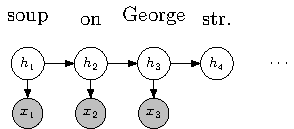
\includegraphics[width=0.5\textwidth]{figures/simple-crf.pdf}
  \end{centering}
  \caption{A conditional random field \todo{(arun): make a CRF and show what happens when measurements are added.}}
\label{fig:crf}
\end{figure}

%Conventionally, we are given a training dataset $\sD = \{\bx_i, \by_i\}$ and can learn $\theta$ by optimizing the convex log-likelihood objective $\sL(\theta) = \sum_{t=1}^T \log \p(\by\oft{t} \given \bx\oft{t})$.
%In our setting, however, we do not observe the gold labels $\by$. 
%Instead, we can ask the crowd to provide a ``measurement'' for some subset of the labels.
%Let $\Sigma = \{\sigma_i\}$ be the set of possible measurements we can ask the crowd for and 
%let $\by_\sigma \subseteq \by$ be the subset of labels queried.

\paragraph{Human error model}
We also model the responses, $z_r$, with an exponential measurement model:
\begin{align*}
  p(z_r \given x, y) 
  &\propto \exp \left( \omega^\top\psi(\bx, y_r, z_r) \right),
\end{align*}
where $\omega$ and $\psi$ are extra parameters and features for the human error model. 
%The choice of an exponential model allows us to simply include measurements as an additional factor.
\figureref{crf} shows the original graph with additional measurement nodes.
A simple human error model is to return the true label with probability $1-\epsilon$ and a random label otherwise.
In our running example, some classes, e.g.\ $\textsc{none}$, are more easily identified than others: in this setting human responses can be modeled to be sampled from a confusion matrix.

Finally, we model delay to be drawn from a Gamma distribution: $\tau_r \sim \Gamma(k, \theta)$\footnote{We assume that the response delays are independent of the input and which label is being queried, though the model can easily be generalized to this setting.}.
The total time taken on a prediction, $\tau$, depends not only on how many requests are made, but also when they are scheduled.
We study the problem of how to best schedule multiple requests in \sectionref{async}.


%In the simplest case, assume the labeler returns the true label with a uniform probability of $1- \epsilon$, and guesses at random otherwise, $\theta'$ and $\phi'$ are:
%\begin{align*}
%  \theta' &= 
%      \begin{bmatrix}
%        1 - \e \\ \e
%      \end{bmatrix} &
%  \phi'(\tau_r, \by_r, \bx) &=
%    \begin{bmatrix}
%      \BI[\tau_r = y_r] \\
%      \BI[\tau_r \neq y_r]
%    \end{bmatrix}.
%\end{align*}
%Independently, we model the time each measurement takes, $D_r$.
%We revisit the problem of learning the error distribution of labelers in \sectionref{human-error}.

Next, we describe how we use our models to predict labels and learn from partial feedback.

\paragraph{Prediction}
Given parameters $\theta, \omega$ and measurement responses $z_1, \ldots, z_n$, we query for predictions using a maximum likelihood labeling:
$\byt \given \bx, z_1, \ldots z_m = \argmax_{\by} \p(\by \given \bx, z_1, \ldots z_n)$.

\paragraph{Learning from responses}

Recall that we do not have gold labels for our data, but only noisy measurements: we do not have supervised examples to learn from. 
As a simple heuristic, we use the output from our model as gold labels and update our parameters periodically.  
In future work, we plan to explore using (online) expectation-maximization to jointly learn parameters for our model and the human error model in an unsupervised fashion.
